\documentclass[11pt,a4paper]{article}
\usepackage{ucs}
\usepackage[T1]{fontenc}
\usepackage[utf8x]{inputenc}
\usepackage[german]{babel}
\usepackage{amsmath}
\usepackage{amsfonts}
\usepackage{amssymb}
\usepackage{graphicx}
\usepackage{shadethm}
\usepackage{caption}
\usepackage{tikz} 
\usepackage{ziffer}
\usepackage{units}
\usepackage{multirow}

\newcommand{\minipanf}{\begin{minipage}{\linewidth}}
\newcommand{\minipend}{\end{minipage}}

\begin{document}

\begin{titlepage}
\newcommand{\HRule}{\rule{\linewidth}{0.5mm}} % Defines a new command for the horizontal lines, change thickness here

\center % Center everything on the page
 
%----------------------------------------------------------------------------------------
%	HEADING SECTIONS
%----------------------------------------------------------------------------------------

\textsc{\LARGE TU Dresden}\\[1.5cm] % Name of your university/college
\textsc{\Large Fortgeschrittenenpraktikum}\\[0.5cm] % Major heading such as course name
\textsc{\Large Praktikumsbericht}\\[0.5cm] % Major heading such as course name

%----------------------------------------------------------------------------------------
%	TITLE SECTION
%----------------------------------------------------------------------------------------

\HRule \\[0.7cm]
{ \huge \bfseries Kernreaktor}\\[0.4cm] % Title of your document
\HRule \\[1.5cm]
 
%----------------------------------------------------------------------------------------
%	AUTHOR SECTION
%----------------------------------------------------------------------------------------

\begin{minipage}{0.4\textwidth}
\begin{flushleft} \large
\emph{Autoren:}\\
Lena \textsc{Schreiner}\\
Toni \textsc{Ehmcke}\\
Christian \textsc{Siegel}
\end{flushleft}
\end{minipage}
~
\begin{minipage}{0.4\textwidth}
\begin{flushright} \large
\emph{Betreuer:} \\
Dr.-Ing. Carsten \textsc{Lange} % Supervisor's Name
\end{flushright}
\end{minipage}\\[4cm]

%----------------------------------------------------------------------------------------
%	DATE SECTION
%----------------------------------------------------------------------------------------

{\large Dresden, \today}\\
\vspace{5mm}
{\large Durchführungstag, 04. Dezember 2015}\\

\vfill 

\end{titlepage} 	% Titelseite

\tableofcontents
\newpage 

\section{Einführung}
	\subsection{Ausbildungskernreaktor AKR-2}
	%TODO: Aufbau, technische Daten im Überblick (vgl erster Link http://tu-dresden.de/die_tu_dresden/fakultaeten/fakultaet_maschinenwesen/iet/wket/akr2/Lehrmaterialien)
	%TODO: Sicherheitsmechanismen (Wann kommt es zu einer RESA?
	\subsection{Kernspaltung}
	%TODO: Kernreaktion, Wirkungsquerschnitt für Neutroneneinfang von U-235 --> Warum benötigt man Moderator? Prompte/verzögerte Neutronen, Lebensdauer
	\subsection{Reaktorkinetik}
	%TODO: Multiplikationsfaktor k, Reaktivität, Reaktorperiode, Verdopplungszeit (nur nennen, nichts herleiten!)
	%TODO: Reaktorkinetische Gleichungen für überkritischen Reaktor + Lösungen --> Wie verhält sich Reaktorleistung bei Reaktivitätsänderung?
	
	\subsection{Steuerstabkalibrierung}
	%TODO: Gleichung für differentielle / integrale Steuerstabkennlinie, INHOUR-Gleichung, Gesamt-, Überschuss-, Abschaltreaktivität.
			% Physikalischer Hintergrund
\section{Durchführung}
    \subsection{Reaktorstart}
    \underline{\textbf{Vor Inbetriebnahme}}  \\ 
    Vor der Inbetriebnahme des Reaktors sind mehrere sicherheitsrelevante Prüfungen an dosimetrischen und nicht-dosimetrischen Einrichtungen vorzunehmen. Zu Beginn werden insbesondere die Anzeigen und Warnsignale auf ihre Funktionalität überprüft, da sie auf Grenzwertüberschreitungen und eine mögliche Reaktorschnellabschaltung hinweisen sollen. Nicht zuletzt wird darüber auch gewährleistet, dass die Messgeräte Signale geben,um als Reaktion darauf eine eventuelle Abschaltung des Reaktors zu verhindern.\\
    Eine RESA findet unter verschiedenen Umständen statt. Zum einen ereignet sie sich bei einer Leistung von weniger als 0,25\unit{W}, da die Neutronenzählrate direkt Proportional zur Leistung sein soll, die statistischen Fehler allerdings bei geringen Leistungen zu groß werden. Einen Warnton erhält man bei 0,3\unit{W}. Zum anderen erfolgt eine RESA durch bei überhöhte Leistung bei 2,4\unit{W}. Einen Warnton erhält man ab 2,2\unit{W}.
    Als Abschaltgrund gilt auch eine zu geringe Reaktorperiode. Während des Versuchs ist als Richtwert eine untere Grenze von 30\unit{s} einzuhalten. Eine Warnung ertönt bei 20\unit{s}, die RESA erfolgt bei 10\unit{s}.
    Ein weiterer Grund für die RESA stellt die Temperatur des Moderators dar. Unterschreitet dieser 22\unit{°C} erfolgt hier eine Abschaltung.\\ \ \\
    \underline{\textbf{Start}}\\
    Ist man sich dieser Grenzwerte bewusst und hat man das akustische Signal gehört, kann fortgefahren werden. Man fährt die Anfahrneutronenquelle ein (ANQ) und beobachtet Änderungen in Leistung und Impulsraten (siehe Tablle \ref{df:ANQein}) . Danach wird überprüft, ob eine manuelle RESA möglich ist. Führt man diese durch, wird die untere Kernhälfte (uKH) abgeworfen. Dies geschieht auch immer genau dann, wenn die oben genannten Grenzwerte erreicht oder überschritten werden. 
    Hat der Abwurf geklappt, kann mit dem Reaktorstart begonnen werden. Man beginnt damit, den RESA-Schalter mittels eines Schlüssels zurückzusetzen, fährt die ANQ in ihre untere Endstellung, fährt die uKH in ihre untere Endstellung. Die Steuerstäbe müssen in der oberen Endstellung stehen. Dies wird durch eine Anzeige, welche so aussieht wie das Schaltzeichen einer Glühlampe, markiert.
    Sind diese Dinge gegeben, kann man den Antrieb der ANQ freigeben und sie in den Reaktor fahren. Sobald sie hineingefahren ist, herrscht ein Mindestneutronenfluss. Dieser ist durch zwei Softwareanzeigen ablesbar: 
    \begin{center}
    \begin{tabular}{l|c|c|c|c}
             Softwareanzeige  & \multicolumn{2}{c|}{\textbf{PHI-WB1}} & \multicolumn{2}{c}{\textbf{PHI-WB2}}\\
                              & Anfang & Endstellung & Anfang & Endstellung \\ 
       \hline           P [mW]& 0,14   & 0,72        & 0,20   & 0,60        \\
         Impulsrate [$s^{-1}$]& 0,3    & 7,5         & 0,4    & 6,3         
    \end{tabular}
    \captionof{table}{Änderung der Leistung und Impulsraten bei Einschub der ANQ}
    \label{df:ANQein}
    \end{center}
    Wenn die uKH in ihrer oberen Endstellung angekommen ist, wird der Anlassschalter auf Ein gesetzt, was die Steuerstäbe einzeln ausfahrbereit macht. Diese werden nun einzeln ausgefahren, bis jeweils eine Reaktorperiode von $\approx$ 30\unit{s} erreicht wird.
    Beim dritten Steuerstab wird nach Abklingen der prompten Neutronen die Verdopplungszeit $T_2$ mittels einer Stoppuhr gemessen. $T_2 = 39\unit{s}$ mit $P_1 = 0,7\unit{W}$ und $P_2 = 1,4\unit{W}$. Der Reaktor ist nun verzögert überkritisch und muss heruntergeregelt werden.\\ \ \\
    \underline{\textbf{Reaktorbetrieb und Dosimetrie}}\\
    Als kritische Leistung soll nun $P=1\unit{W}$ eingestellt werden. Ist dieser Wert erreicht, wird er konstant mithilfe der Nachkalibrierung des 3. Steuerstabs gehalten, währenddessen dosimetrische Messungen vorgenommen werden. Sind diese Messungen abgeschlossen werden sie bei einer Leistung von $P = 2\unit{W}$ an den gleichen Stellen wiederholt.
    Als abschließende Steuerstabpositionen erhält man $x_{1\unit{W}} = 2238$ und $x_{2\unit{W}} = 2250$ bei einer konstanten Temperatur von 22,4\unit{°C}. Dies scheint verhältnismäßig konstant und mit der Temperatur des Moderators korelliert zu sein.
    \begin{center}
        \begin{tabular}{l|c|c|c|c}
                \textbf{Ort} & \multicolumn{2}{c|}{\textbf{bei 1\unit{W}}} & \multicolumn{2}{c}{\textbf{bei 2\unit{W}}} \\
       \hline       & $\dot D_\gamma$ [\textit{$\mu Sv/h$}] & $\dot D_n$ [\textit{$\mu Sv/h$}]& $\dot D_\gamma$ [\textit{$\mu Sv/h$}]& $\dot D_n$ [\textit{$\mu Sv/h$}]\\
       \hline   Reaktortankwand ($\approx \unit[0]{m}$) & 12 & 2,5 & 27,5 & 4,3 \\
                Operatortisch ($\approx \unit[3]{m}$) & 1,4 & 0,2 & 2,5 & 0,6 \\
                Ecke ($\approx \unit[6]{m}$) & 0,6 & 0,14 & 0,5 & 0,13 
        \end{tabular}
        \captionof{table}{Dosimetrische Messung von Neutronen und Photonen an verschiedenen Orten und mit unterschiedlichen Leistungen}
        \label{dft:dosi}
        \begin{figure}[H]
            \subfigure[Dosisleistung von Neutronen\label{p:dosi_neu}]{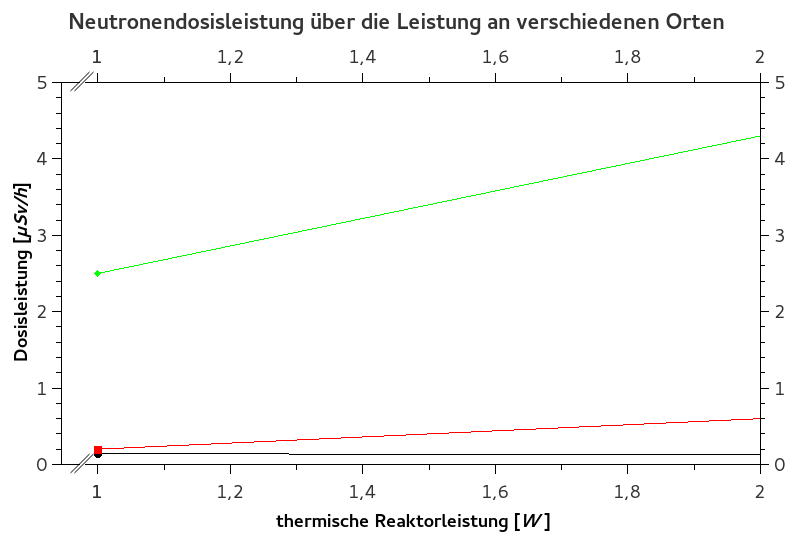
\includegraphics[scale=0.35]{pic/neutronendosisleistung}}
            \subfigure[$\gamma$-Dosisleistung\label{p:dosi_gamma}]{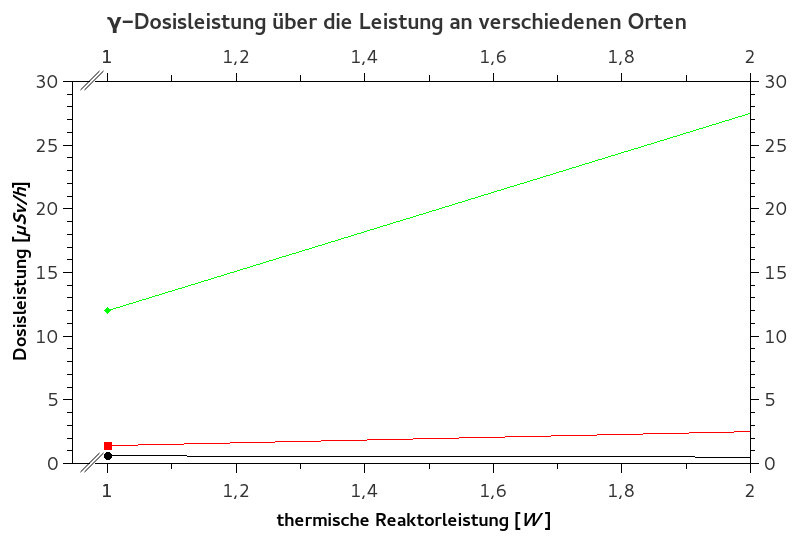
\includegraphics[scale=0.35]{pic/gamma_dosisleistung}}
            \caption{Dosisleistungen bei verschiedenen Reaktorleistungen}
            \label{df:dosi_g_n}                    
        \end{figure}
    \end{center}
        \begin{figure}[H]
            \centering
            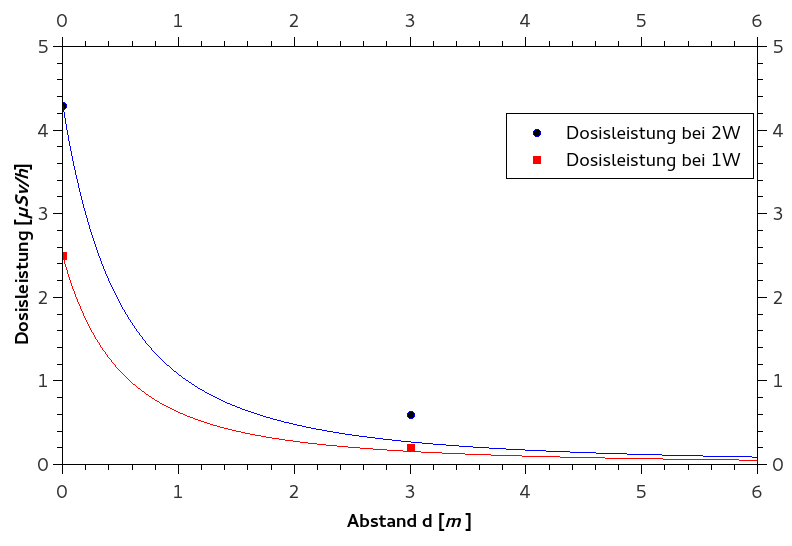
\includegraphics[scale=0.5]{pic/Neutronendosisleistung_Abstand}
            \caption{Dosisleistung der Neutronenstrahlung an verschiedenen Orten bei unterschiedlichen thermischen Leistungen}
            \label{df:neu_abstand}
        \end{figure}

    \ \\    
    Aus Tabelle \ref{dft:dosi} lässt sich für Neutronen das Abstandsquadratgesetz herleiten. Der direkt proportionale Zusammengang zwischen thermischer Reaktorleistung und der Dosisleistungen von Neutronen und 

    \subsection{Steuerstabkalibrierung}

			% Durchführung
\section{Zusammenfassung und Diskussion}
	Im Experiment wurde sich mit den Grundlagen der Bedienung eines Kernreaktors vertraut gemacht. Dabei wurden zunächst die notwendigen einführenden Sicherheitsmaßnahmen zur Gewährleistung der nuklearen Sicherheit durchgeführt. Anschließend wurde die vorherrschende Dosisleistung an unterschiedlichen Orten und in Abhängigkeit der Reaktorleistung ermittelt. Dabei wurde das \textit{Abstandsquadratsgesetz} bestätigt, das heißt, dass die Dosisleistung mit dem Quadrat des Abstands zur Quelle sinkt (Abbildung \ref{df:neu_abstand}). Weiterhin wurde festgestellt, dass die Dosisleistung der Neutronen- und $\gamma$-Strahlung linear mit der Reaktorleistung zunimmt (Abbildungen \ref{p:dosi_neu} und \ref{p:dosi_gamma}). Die aufgenommenen Messdaten hätten verbessert werden können, indem man wesentlich mehr Messpunkte aufgenommen hätte.\\
	Im zweiten Teil des Experimentes wurde eine Kalibrierung der Steuer- und Regeleinrichtungen am AKR über ein Kompensationsverfahren vorgenommen. Dafür wurde die Reaktorperiode ermittelt und mit Hilfe der Inhour-Gleichung (\ref{int:inhour}) die differentielle Reaktivität bestimmt. Mit Hilfe der daraus ableitbaren integralen Steuerstabkennlinie wurde die Überschussreaktivität des AKR-2 mit $ \rho_{\ddot{U}berschuss}  = (0,64 \pm 0,03)\ \unit{\$}$ quantifiziert. Da dieser Wert kleiner als $1\ \unit{\$}$ ist, kann weder durch technische noch durch personelle Fehler ein prompt überkritischer Reaktorzustand erreicht werden, weshalb das AKR als sehr sicherer Reaktor eingestuft werden kann. Der oben genannte Messwert könnte genauer ermittelt werden, indem man die Zeitmessung der Reaktorperiode entweder häufiger mit mehreren unabhängigen Stoppuhren vornimmt oder man die Messung der Verdopplungszeit automatisiert.\\
	Im letzten Teil des Experiments wurde die Reaktivität einer Cadmium-Probe mit $\rho_{Cd}\prime = (0,13 \pm 0,02)\ \unit{\$}$ bestimmt. Da der ermittelte Wert aus der integralen Steuerstabkennlinie durch bloßes Ablesen extrahiert wurde, könnte die Genauigkeit erhöht werden, indem man diese numerisch fittet.
		% Auswertung
\begin{thebibliography}{99}
\bibitem [01] {stab} Technische Universität Dresden,  Institut für Energietechnik Ausbildungskernreaktor: \textit{Reaktorpraktikum Versuch "Steuerstabskalibrierung"}. Dresden, 05/2011 
\bibitem [02] {start}Technische Universität Dresden,  Institut für Energietechnik Ausbildungskernreaktor: \textit{Reaktorpraktikum Versuch "Reaktorstart"}. Dresden, 05/2011
\bibitem [03] {Wirkungsquerschnitt_Uran} A. Ganczarczyk: \textit{Physikalische Grundlagen der Energieumwandlung}. \texttt{https://www.uni-due.de}. Duisburg, 01/2006, zuletzt geöffnet: 10.01.2016
\bibitem [04] {Flyer}Technische Universität Dresden, Institut für Energietechnik Ausbildungskernreaktor: \textit{Flyer Ausbildungskernreaktor}
\bibitem [05] {Aufbau} Technische Universität Dresden, Institut für Energietechnik Ausbildungskernreaktor: \textit{Ausbildungskernreaktor AKR-2 Beschreibung des Aufbaus, der Funktionskontrolle und der Betriebsprotokollierung der Reaktoranlage AKR-2}. Dresden, 2005

\end{thebibliography}



\end{document}
